Through this manual, we learn how to measure an unknown resistance through arduino and display it on an LCD.
\begin{enumerate}[label=\arabic*.,ref=\theenumi]
%
\item
Let $R_1$ be the known resistor and $R_2$ be the unknown resistor.  Connect $R_1$ and $R_2$ in series such that $R_1$ is connected
to GND and $R_2$ is connected to $V_{cc}$. Refer to Fig. \ref{fig:voltage_divider}

%
%
		\begin{figure}[!htb]
\centering
\resizebox {0.5\columnwidth} {!} {
\begin{circuitikz}[american]
      \draw (0,2) node[ocirc,label={[font=\footnotesize]below:$V_{CC}$}] {}
%      to[V=$V_{CC}$, invert] (0,2) % The voltage source
%      to[short] (2,2)
    to[R=$R_1 (known)$] (2,2) % The resistor
      to[R=$R_2 (unknown)$] (2,0)
      to (2,-0.5) node[ground]{GND}      ; % The resistor
%      to[short] (0,0);
\draw (2,2)   to [short, -o]   (4,2) node[label={[font=\footnotesize]above:$A0$}] {};
%\draw (2,0)   to [short, -o]   (4,0);
%\draw (2,-0.5) node[ground]{GND}  to[short] (2,0);
\end{circuitikz}

%\begin{circuitikz}[american]
%      \draw (0,0)
%      to[V=$V_{CC}$, invert] (0,2) % The voltage source
%%      to[short] (2,2)
%    to[R=$R_1$] (2,2) % The resistor
%      to[R=$R_2$] (2,0) % The resistor
%      to[short] (0,0);
%\draw (2,2)   to [short, -o]   (4,2) node[label={[font=\footnotesize]above:$A3$}] {};
%%\draw (2,0)   to [short, -o]   (4,0);
%\draw (2,-0.5) node[ground]{GND}  to[short] (2,0);
%\end{circuitikz}

}
\caption{Voltage Divider}
\label{fig:voltage_divider}
\end{figure}
%

\item
Connect the junction between the two resistors to  the A0 pin on the Arduino.

%
\item
Connect the arduino to the computer so that it is powered.

%
\item
Open the Arduino IDE and type the following code.  Open the {\em serial monitor} to view the output.

%
		\begin{lstlisting}
ide/lcd/codes/resistance/resistance.ino
		\end{lstlisting}
%
\item Plug the LCD in Fig. \ref{fig:avr-gcc/lcd/lcd} to the breadboard.
\iffalse
%
\begin{figure}
\centering
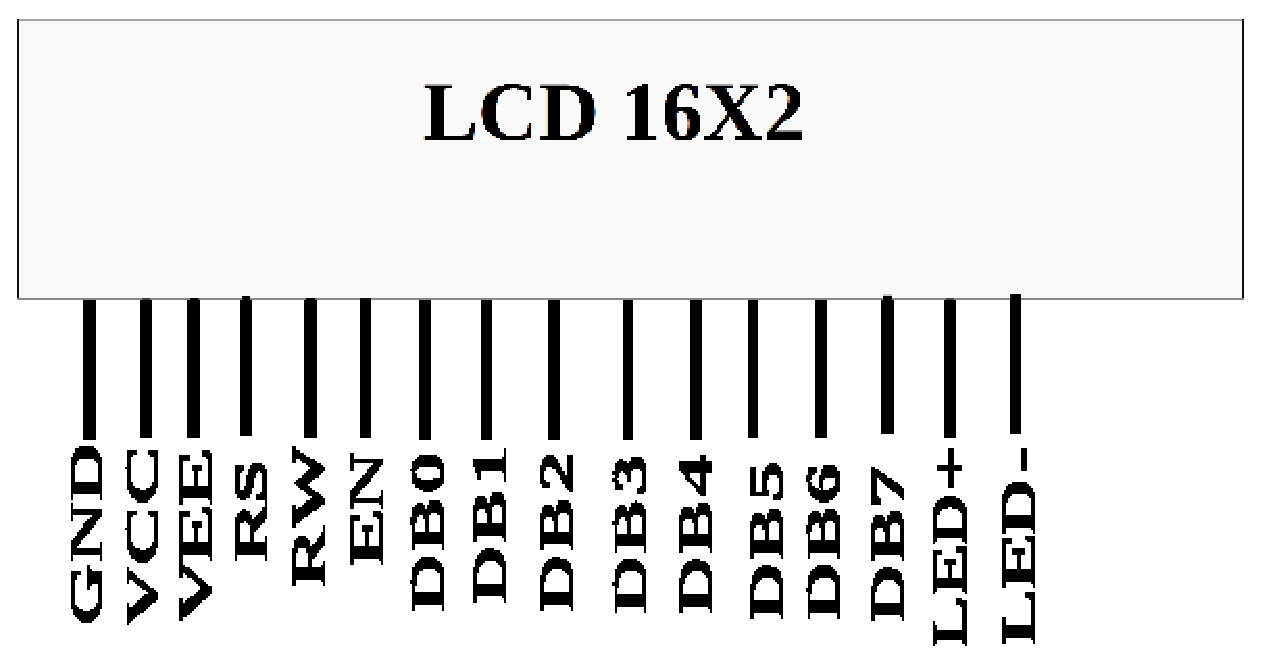
\includegraphics[width=0.75\columnwidth]{ide/lcd/figs/lcd}
\caption{lcd}
\label{fig:lcd}
\end{figure}
\fi
%
\item
Connect the 220$\Omega$ resistance from $V_{cc}$ to pin 15 (Led+) of the LCD.

%
%%
%\item
%Connect  pin 16 (Led-) of the LCD to GND.  The LCD should glow.
%
%%
%\item
%Connect pin 3 of the LCD to GND.  This is required for contrast.
%
\item
Connect the Arduino pins to LCD pins as per Table \ref{table:lcd pins}.
%
\item
Include the instructions for the LCD in the code for measuring the resistance. 
\solution 
%
		\begin{lstlisting}
ide/lcd/codes/lcd/resistance_lcd.ino
		\end{lstlisting}
\item We create a variable called analogPin and assign it to 0. 
This is because the voltage value we are going to read is connected to analogPin A0.
\item  The 10-bit ADC can differentiate 1024 discrete voltage levels, 5 volt is applied to 2 resistors and the voltage sample is taken in between the resistors. The value which we get from analogPin can be between 0 and 1023. 0 would represent 0 volts falls across the unknown resistor. A value of 1023 would mean that practically all 5 volts falls across the unknown resistor.
\item  $V_{out}$ represents the divided voltage that falls across the unknown resistor.
\item  The Ohm meter in this manual works on the principle of the voltage divider shown in Fig. \ref{fig:voltage_divider}.
%
\begin{align}
V_{out}&=\frac{R_1}{R_1+R_2}V_{in} \\
\Rightarrow R_2&=R_1\brak{\frac{V_{in}}{V_{out}}-1}
\end{align}
%
In the above, $V_{in} = 5$V, $R_1 = 220 \Omega$.
\end{enumerate}



